%%%%%%%%%%%%%%%%%%%%%%%%%%%%%%%%%%%%%%%%%
% Developer CV
% LaTeX Template
% Version 1.0 (28/1/19)
%
% This template originates from:
% http://www.LaTeXTemplates.com
%
% Authors:
% Jan Vorisek (jan@vorisek.me)
% Based on a template by Jan Küster (info@jankuester.com)
% Modified for LaTeX Templates by Vel (vel@LaTeXTemplates.com)
%
% License:
% The MIT License (see included LICENSE file)
%
%%%%%%%%%%%%%%%%%%%%%%%%%%%%%%%%%%%%%%%%%

%----------------------------------------------------------------------------------------
%	PACKAGES AND OTHER DOCUMENT CONFIGURATIONS
%----------------------------------------------------------------------------------------

\documentclass[9pt]{developercv} % Default font size, values from 8-12pt are recommended


%----------------------------------------------------------------------------------------

\begin{document}

%----------------------------------------------------------------------------------------
%	TITLE AND CONTACT INFORMATION
%----------------------------------------------------------------------------------------

\begin{minipage}[t]{0.45\textwidth} % 45% of the page width for name
	\vspace{-\baselineskip} % Required for vertically aligning minipages
	
	% If your name is very short, use just one of the lines below
	% If your name is very long, reduce the font size or make the minipage wider and reduce the others proportionately
	\colorbox{black}{{\huge\textcolor{white}{\textbf{\MakeUppercase{Jonas}}}}} % First name
	
	\colorbox{black}{{\huge\textcolor{white}{\textbf{\MakeUppercase{Schultheiss}}}}} % Last name
	
	\vspace{6pt}
	
	{\huge Full stack developer} % Career or current job title
\end{minipage}
\begin{minipage}[t]{0.32\textwidth} % 27.5% of the page width for the first row of icons
	\vspace{-\baselineskip} % Required for vertically aligning minipages
	
	% The first parameter is the FontAwesome icon name, the second is the box size and the third is the text
	% Other icons can be found by referring to fontawesome.pdf (supplied with the template) and using the word after \fa in the command for the icon you want
	\icon{MapMarker}{12}{Ettingen, Schweiz}\\
	\icon{Phone}{12}{+41 76 747 61 55}\\
	\icon{At}{12}{\href{mailto:contact@jonasschultheiss.dev}{contact@jonasschultheiss.dev}}\\	
\end{minipage}
\begin{figure}[!ht]
  \centering
  \colorbox{black}{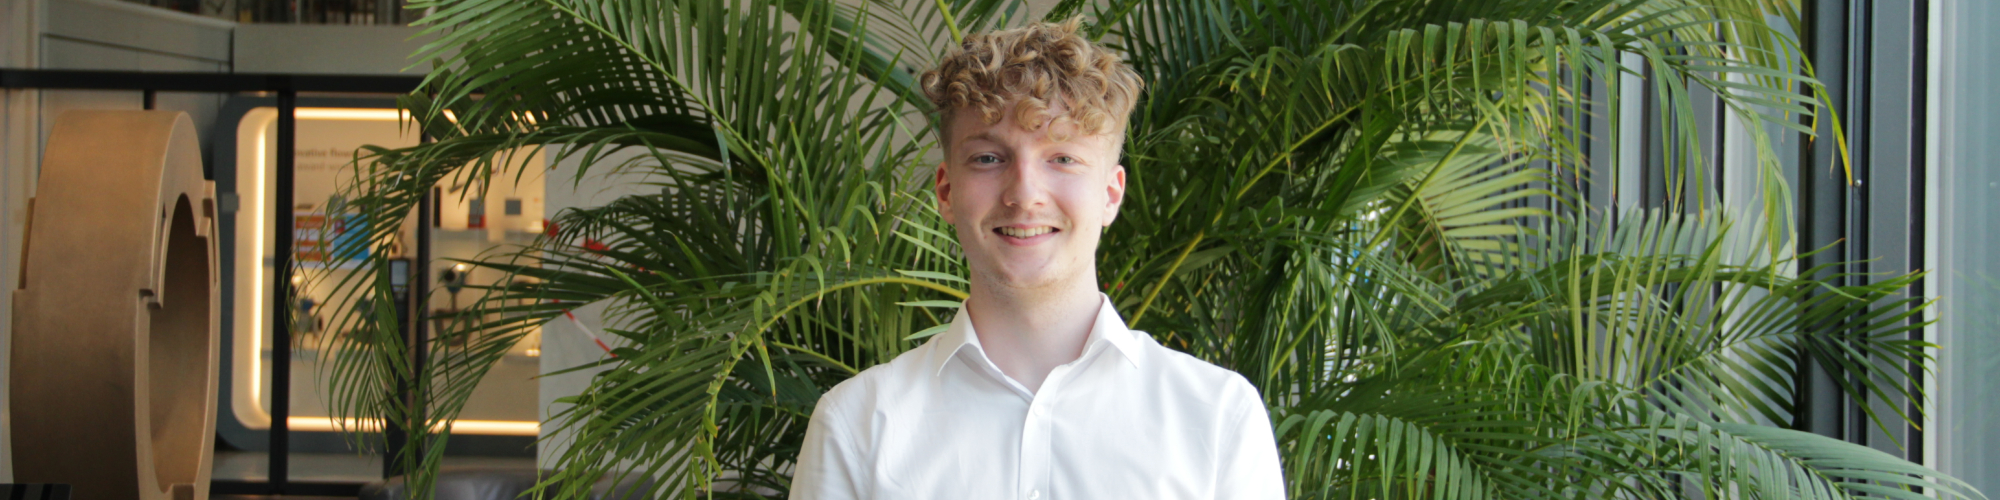
\includegraphics[width=1\linewidth]{./me.jpg}}
\end{figure}
\begin{minipage}[t]{0.23\textwidth} % 27.5% of the page width for the second row of icons
	\vspace{-\baselineskip} % Required for vertically aligning minipages
	
	% The first parameter is the FontAwesome icon name, the second is the box size and the third is the text
	% Other icons can be found by referring to fontawesome.pdf (supplied with the template) and using the word after \fa in the command for the icon you want
	\icon{Globe}{12}{\href{https://jonasschultheiss.dev}{jonasschultheiss.dev}}\\
	\icon{Github}{12}{\href{https://github.com/jonasschultheiss}{jonasschultheiss}}\\
	\icon{Twitter}{12}{\href{https://twitter.com/@SchultheissJ}{@SchultheissJ}}\\
\end{minipage}

\vspace{0.5cm}

%----------------------------------------------------------------------------------------
%	INTRODUCTION, SKILLS AND TECHNOLOGIES
%----------------------------------------------------------------------------------------

\cvsect{Summary}

\begin{minipage}[t]{0.48\textwidth} % 40% of the page width for the introduction text
	\vspace{-\baselineskip} % Required for vertically aligning minipages
  I am a full stack developer from Switzerland, currently employed as an apprentice at Endress+Hauser until the end of July 2021. Endress+Hauser is the market leader for measuring instruments used in industry. Its portfolio also includes the IIoT platform "Netilion", the offer of complete solutions and various services. I always did more than expected of me throughout this placement, both in terms of college work and work-based tasks.
\end{minipage}
\hfill % Whitespace between
\begin{minipage}[t]{0.48\textwidth} % 50% of the page for the skills bar chart
	\vspace{-\baselineskip} % Required for vertically aligning minipages
  This foundation has provided me with a solid technical skill set and work based experience in preparation for a career in computer science.

  My current main stack consists of Next.js and Nest.js but this can vary from project to project.
  
  I am interested in working as a full stack developer in a progressive company that values teamwork, communication and modern technologies. It is important to me that I am offered the opportunity to actively further my education so that I stay up to date in web development.
\end{minipage}

% \begin{center}
% 	\bubbles{5/Eclipse, 6/git, 4/Office, 3/Inkscape, 3/Blender}
% \end{center}

%----------------------------------------------------------------------------------------
%	EXPERIENCE
%----------------------------------------------------------------------------------------

\cvsect{WORK EXPERIENCE}

\begin{entrylist}
	\entry
		{08.2017 -- 07.2021}
		{IT Apprentice EFZ, field of study application development}
		{\href{https://endress.com}{Endress+Hauser Process Solutions AG}}
		{In summer 2017, I started my apprenticeship as a computer scientist specialising in application development at Endress+Hauser. In the Swiss apprenticeship system, you have one or two days of vocational school per week. The rest is spent within the company. The first year of the apprenticeship provided a basic foundation in computer science. In the company, I was taught C\# intensively by my line manager.

    In the second year of my apprenticeship, I focused on JavaScript. I was given the task by my employer to replace the existing Bash scripts with a Node.js application that was used in the production of a device or its software. The Bash scripts were old, difficult to maintain and slow. This project allowed me to build a solid foundation in JavaScript and Node.js and made the system easier to use for the team.
    
    During the third year of my apprenticeship, I became heavily involved with web development. I used React and to create several websites used in training and/or sales to make the IIoT attractive and more understandable to customers. I also worked together with the web development team for several months. During this time, I created a website where the customer can interact with a 3D model. You can find more about this on my portfolio site.\\ \texttt{Next.js}\slashsep\texttt{Nest.js}\slashsep\texttt{C\#}}
\end{entrylist}
%----------------------------------------------------------------------------------------
%	EDUCATION
%----------------------------------------------------------------------------------------

\cvsect{EDUCATION}

\begin{entrylist}
	\entry
		{08.2017 -- 07.2021}
		{IT Apprentice EFZ, field of study application development}
		{\href{https://www.bbzbl.ch/}{BBZ-BL}}
		{During my training, I attended the BBZ-BL. Here I received my basic training in computer science. Various school projects can be found on my website.}
	\entry
		{06.2012 -- 08.2017}
		{Compulsory education, secondary school level E}
		{\href{https://www.sektherwil.ch/}{Sekundarschule Therwil}}
		{}
\end{entrylist}
\pagebreak

%----------------------------------------------------------------------------------------
%	Additional experiences
%----------------------------------------------------------------------------------------

\cvsect{ADDITIONAL EXPERIENCES}

\begin{entrylist}
	\entry
		{10.2020}
		{E+H PCPS Fedex Day 2020}
		{\href{https://endress.com}{Endress+Hauser Process Solutions AG}}
		{This was the third hackathon I participated in, we used embedded components coupled with a Node.js Script and Backend and a React Frontend to give employees the opportunity to control their desk lamps. With the embedded interface we controlled the brightness and warmth of the lamp. The plan was to make this into a full internal project, where an employee could make their own profile, which can change the warmth based on the time of the day. However, it is currently unclear whether the company will turn it into a full project.\\ \texttt{React}\slashsep\texttt{Node.js}}
	\entry
		{12.09.2020}
		{ICTskills2020: The Swiss Championships in the ICT Vocational Field}
		{\href{https://www.ict-berufsbildung.ch/}{ICT-Berufsbildung Schweiz}}
		{The ICTSkills are the Swiss professional championships in the IT sector. After successfully qualifying in regional rounds, I took part in the national competition in Bern.

    In one day we had to solve various challenges in HTML, CSS, JavaScript, ReGeX, PHP and MySQL. I succeeded quite well. Unfortunately, I had to give up almost all PHP points, as I didn't focus on PHP during the apprenticeship, but on Node.js.
    Nevertheless, I learned a lot, especially ReGeX, through the preparation and the professional championship and deepened what I had already learned.\\ \texttt{HTML5}\slashsep\texttt{CSS3}\slashsep\texttt{JavaScript}\slashsep\texttt{ReGeX}\slashsep\texttt{PHP}\slashsep\texttt{SQL}}
	\entry
		{10.2019 -- 11.2019}
		{C++ Workshop}
		{\href{https://ethz.ch/}{ETH Zürich}}
		{This two-weekend C++ workshop was led by students from ETH Zurich. Various challenges had to be solved, in which the runtime and the size of the working memory had to be taken into account. The students explained more about C++, the Big O notation and other concepts in theory blocks.
    I was able to learn a lot from this.\\ \texttt{C++}}
	\entry
		{10.2019}
		{E+H PCPS Fedex Day 2019}
		{\href{https://endress.com}{Endress+Hauser Process Solutions AG}}
		{The second hackathon I participated in. We improved the prototype from last years hackathon. We built it again from scratch, but used our experience from the previous year. The biggest difference to last year was, that we replaced the express.js backend with the Firebase Realtime Database from Google. This allowed us to directly update a value or react to a change without needing to build the structure for it.\\ \texttt{React}\slashsep\texttt{Firebase}}
	\entry
		{10.2018}
		{E+H PCPS Fedex Day 2018}
		{\href{https://endress.com}{Endress+Hauser Process Solutions AG}}
		{The first hackathon I have participated in. We created a prototype for an IoT system that measures the air quality in meeting rooms and displays it on a website.\\ \texttt{Node.js}\slashsep\texttt{MongoDB}}
	\entry
		{09.2018 -- 11.2018}
		{AppQuest}
		{\href{https://appquest.ch/}{Hochschule für Technik Rapperswil and Berner Fachhochschule}}
		{Mobile development course with swift. We got a diverse set of challenges. To overcome these challenges you had to code various small apps. An example would be an app that laid a red filter over the output of the camera, so you could read hidden messages in a picture.

    We made these Apps because they were needed for a treasure hunt. There we got hints that could only be read if you correctly programmed your app.\\ \texttt{Swift}\slashsep\texttt{iOS}}
\end{entrylist}

%----------------------------------------------------------------------------------------
%	ADDITIONAL INFORMATION
%----------------------------------------------------------------------------------------

\begin{minipage}[t]{0.3\textwidth}
	\vspace{-\baselineskip} % Required for vertically aligning minipages

	\cvsect{LANGUAGES}
	
	\textbf{German} - Native proficiency\\
	\textbf{English} - Full professional proficiency\\
\end{minipage}
\hfill
\begin{minipage}[t]{0.3\textwidth}
	\vspace{-\baselineskip} % Required for vertically aligning minipages
	
	\cvsect{HOBBIES}
	
	In my free time, I like to play football, volleyball or basketball with my colleagues. I also I like to spend my time with my little brother.
\end{minipage}
\hfill
\begin{minipage}[t]{0.3\textwidth}
	\vspace{-\baselineskip} % Required for vertically aligning minipages
	
	\cvsect{Non profit}
	
  Together with friends and acquaintances, I founded the non-profit club "PR1SM", which is actively involved in digital media and regional e-sports.
\end{minipage}

%----------------------------------------------------------------------------------------

\end{document}
